\newpage
\section{Gerjesztett rezgőrendszerek}

\subsection*{Nagyítási- és fáziskésés diagramok}
A harmonikusan gerjesztett, egy szabadsági fokú rendszerek frekvencia-válaszát mutatják be ezek az ábrák.

A tengelyeken szereplő mennyiségek jelentése:
\begin{itemize}
    \item \textbf{Vízszintes tengely ($\lambda = \frac{\omega}{\omega_n}$):} Relatív (vagy hangolási) frekvencia. A gerjesztő körfrekvencia és a sajátkörfrekvencia hányadosa.
    \item \textbf{Függőleges tengely (Nagyítási diagram, $N$):} Dinamikus nagyítási tényező (amplitúdóviszony). Megmutatja, milyen mértékben növeli a dinamika a statikus deformációt (az $x_{stat}$ kitérést).
    \item \textbf{Függőleges tengely (Fáziskésés diagram, $\vartheta$):} Fáziskésési szög. A gerjesztő erő harmonikus menete és a fellépő elmozdulás közötti időbeli eltolódást fejezi ki (fokban vagy radiánban).
\end{itemize}

\begin{figure}[H]
    \centering
    \begin{minipage}{0.48\textwidth}
        \centering
        \textbf{Nagyítási diagram ($N-\lambda$)} \\
        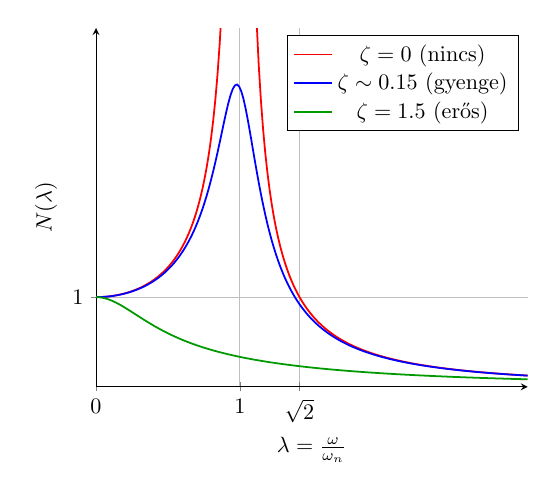
\begin{tikzpicture}[scale=0.8]
            \begin{axis}[
                axis lines=left,
                xlabel={$\lambda = \frac{\omega}{\omega_n}$},
                ylabel={$N(\lambda)$},
                xmin=0, xmax=3,
                ymin=0, ymax=4,
                xtick={0, 1, 1.414},
                xticklabels={0, 1, $\sqrt{2}$},
                ytick={1},
                grid=both,
                samples=200, domain=0:3,
                restrict y to domain=0:5
            ]
                % Undamped (zeta=0)
                \addplot[thick, red] {abs(1/(1-x^2))};
                % Underdamped (zeta=0.15)
                \addplot[thick, blue] {1/sqrt((1-x^2)^2 + (2*0.15*x)^2)};
                % Overdamped (zeta=1.5)
                \addplot[thick, green!60!black] {1/sqrt((1-x^2)^2 + (2*1.5*x)^2)};
                
                \legend{$\zeta=0$ (nincs), $\zeta \sim 0.15$ (gyenge), $\zeta=1.5$ (erős)}
            \end{axis}
        \end{tikzpicture}
    \end{minipage}\hfill
    \begin{minipage}{0.48\textwidth}
        \centering
        \textbf{Fáziskésés diagram ($\vartheta-\lambda$)} \\
        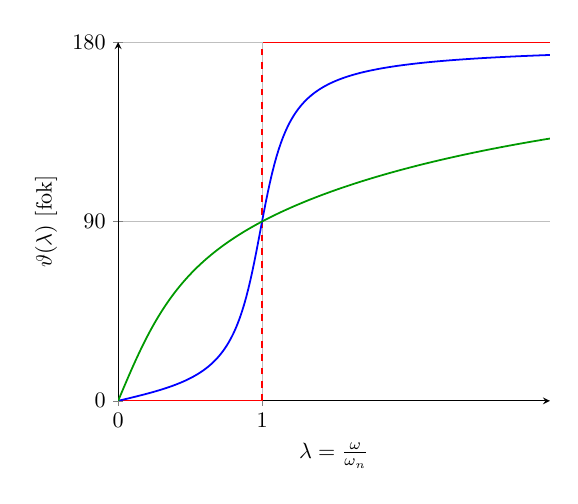
\begin{tikzpicture}[scale=0.8]
            \begin{axis}[
                axis lines=left,
                xlabel={$\lambda = \frac{\omega}{\omega_n}$},
                ylabel={$\vartheta(\lambda)$ [fok]},
                xmin=0, xmax=3,
                ymin=0, ymax=180,
                xtick={0, 1},
                xticklabels={0, 1},
                ytick={0, 90, 180},
                grid=both,
                samples=200, domain=0:3
            ]
                % Undamped (zeta=0)
                \addplot[thick, red, domain=0:0.99] {0};
                \addplot[thick, red, domain=1.01:3] {180};
                \draw[thick, red, dashed] (axis cs:1,0) -- (axis cs:1,180);
                
                % Underdamped (zeta=0.15)
                \addplot[thick, blue] {
                    x<=1 ? atan((2*0.15*x)/(1-x^2)) : 180+atan((2*0.15*x)/(1-x^2))
                };
                
                % Overdamped (zeta=1.5)
                \addplot[thick, green!60!black] {
                    x<=1 ? atan((2*1.5*x)/(1-x^2)) : 180+atan((2*1.5*x)/(1-x^2))
                };
            \end{axis}
        \end{tikzpicture}
    \end{minipage}
    \caption{Nagyítási és fáziskésési diagramok nevezetes pontokkal (rezonancia a $\lambda \approx 1$ környezetében, izolációs szakasz $\lambda>\sqrt{2}$ felett).}
\end{figure}

\newpage
\subsection*{Mozgástörvény összetevői és kapcsolata a nagyítási diagrammal}
Egy csillapított, harmonikusan gerjesztett rendszer mozgása két összetevő szuperpozíciójából áll: az általános (homogén) és a partikuláris megoldásból, amiket a tranziensek és állandósult nevekkel is jelölnek. A \textbf{tranziens szakasz} kezdetben szabálytalan burkolót ad és folyamatosan lecseng, majd ezt teljesen dominánsan felváltja a \textbf{stacionárius rezgés}, ami a rendszer kizárólagos gerjesztés hatására történő színtiszta együttmozgása.

\begin{figure}[H]
    \centering
    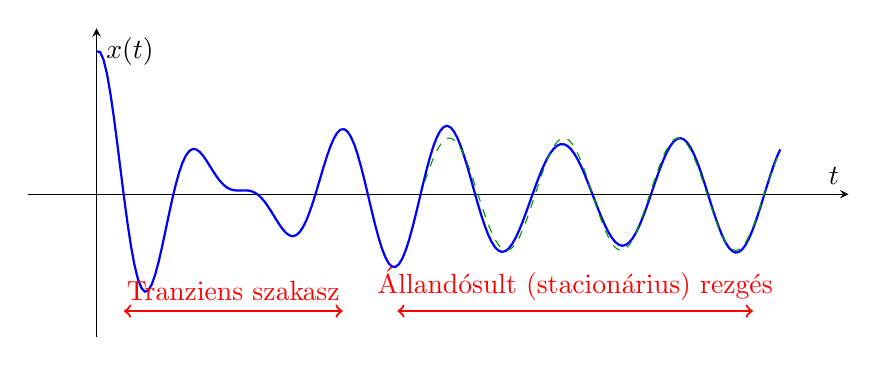
\begin{tikzpicture}
        \begin{axis}[
            width=12cm, height=5.5cm,
            axis lines=middle,
            xlabel={$t$},
            ylabel={$x(t)$},
            xmin=0, xmax=25,
            ymin=-2.5, ymax=3,
            xtick=\empty, ytick=\empty,
            enlargelimits=0.1,
            samples=200,
            domain=0:25
        ]
            % Total: Homogenous + Particular
            \addplot[thick, blue] { 2*exp(-0.15*x)*cos(deg(1.99*x)) + 1.2*cos(deg(1.5*x - 0.5)) };
            % Highlight steady state
            \addplot[dashed, green!60!black, domain=12:25] { 1.2*cos(deg(1.5*x - 0.5)) };
            
            \draw[<->, thick, red] (1, -2.5) -- (9, -2.5) node[midway, above] {Tranziens szakasz};
            \draw[<->, thick, red] (11, -2.5) -- (24, -2.5) node[midway, above] {Állandósult (stacionárius) rezgés};
        \end{axis}
    \end{tikzpicture}
    \caption{A mozgástörvény tranziens és stacionárius alkatrészei időbeni szétválasztásban.}
\end{figure}

\textbf{A mozgástörvény és a nagyítási diagram kapcsolata:} \\
Gyakorlati szempontból a nagyítási diagram ($N-\lambda$) szigorúan csak ezt az \textbf{állandósult (stacionárius)} szakaszt írja le. Az $N(\lambda)$ ordínáta meg is adja, hogy az állandósult rezgés amplitúdója ($X = x_{stat} \cdot N$) hányszorosa a statikus kitérésnek, ami a mechanikai méretezéshez kritikus fontosságú peremfeltételt reprezentál. A tranziens rezgés gyors csillapodás általi eltűnése után rendszerünk már kizárólag ezen az explicit nagyítási görbén lévő $N$ tényezővel, és egy harmonikus fáziskéséssel ($\vartheta$) fog rezegni.
